\begin{figure}[h]
    \centering
    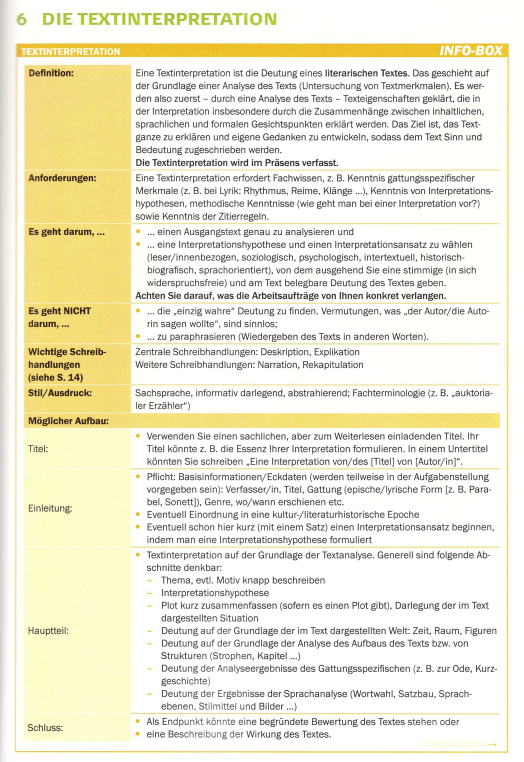
\includegraphics[scale=0.8]{./pics/Screenshot from 2023-02-06 12-31-18.png}
    \caption{Textinterpretation: Definition + Aufbau}
    \label{fig:impl:Textinterpretation1}
\end{figure}

\begin{figure}[h]
    \centering
    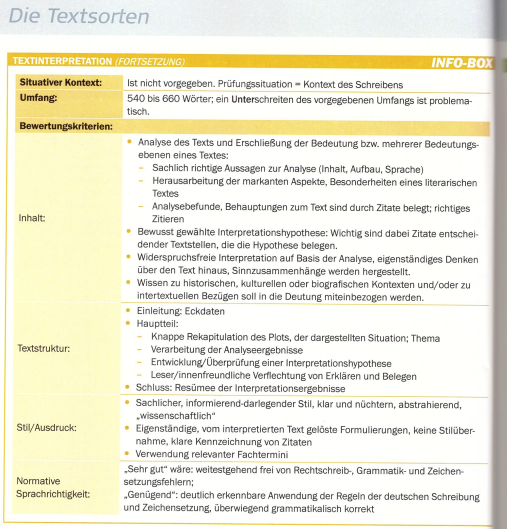
\includegraphics[scale=0.8]{./pics/Screenshot from 2023-02-06 12-31-28.png}
    \caption{Textinterpretation: Verfassen}
    \label{fig:impl:Textinterpretation2}
\end{figure}
\begin{figure}[h]
    \centering
    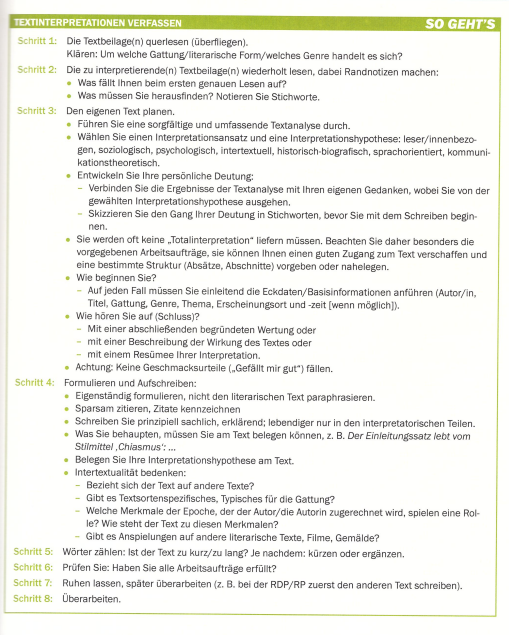
\includegraphics[scale=0.8]{./pics/Screenshot from 2023-02-06 12-32-23.png}
    \caption{Textinterpretation: Fortsetzung}
    \label{fig:impl:Textinterpretation3}
\end{figure}



\section{Mustertext}

\subsubsection{Nichts ist unpräziser als Gerechtigkeit }
Eine Interpretation von „Lieferung frei Haus“ von Günter Kunert 

In der Kurzgeschichte „Lieferung frei Haus“, die 1988 in „Arbeitstexte für den Deutschunterricht. Deutsche Kurzgeschichten 11. – 13. Schuljahr“ erschien, beschreibt Günter Kunert die Tücken einer Welt, in der absolute Gerechtigkeit herrscht, und stellt gleichzeitig die Frage, ob man einen Menschen für alle Folgen seines Handelns verantwortlich machen kann.  

Anfangs wird beschrieben, wie anonyme Lastwägen in der Dämmerung Holzkisten an verschiedenste Haushalte ausliefern. Dies geschieht auch im Haus, in dem Friedrich W. Schmall, der Hauptcharakter, wohnhaft ist. Im Vorbeigehen bemerkt er den Empfänger, der diese Lieferung voller Entsetzen entgegennimmt. Schmall wird schon bald von der Portiersfrau aufgeklärt, beim Inhalt der Kisten handle es sich um Leichen. Dieses absurde Vorkommnis wird ihm von der Bäckersfrau bestätigt, deren Mann ebenfalls eine Leiche in Empfang nehmen musste. Es handelt sich um eine Greisin, die dieser auf regennasser Straße mit seinem Auto tötete. Schmall kann sich einen Anflug von Freude über diese ausgleichende Gerechtigkeit nicht verkneifen. Auf der Straße trifft er auf eine Menschenmenge, die beobachtet, wie ein Ex-Soldat, der Deserteure erschoss, vierzig Kisten geliefert bekommt. Danach bekommt Schmall erstmals Zweifel an den Akteuren und der moralischen Rechtfertigung hinter diesen Lieferungen. Als er seine Verlobte besuchen will, bekommt auch sie eine solche Lieferung. Er flüchtet, ohne mit ihr zu sprechen. Als er sie später darauf anspricht, rechtfertigt sie sich, doch er flüchtet wieder. Die Geschichte endet damit, dass auch Friedrich W. Schmall eine Holzkiste geliefert bekommt, die seine Verlobte beinhaltet. Sie konnte den Verlust ihres Mannes nicht verkraften und nahm sich das Leben.  

Die Kurzgeschichte ist aus der Perspektive eines personalen Erzählers geschrieben, der die Handlung linear wiedergibt und stets im Präteritum bleibt. Sprachlich fallen besonders die Beschreibungen der Personen auf, besonders die Beschreibungen der Empfänger der Holzkisten im Moment der Übergabe sind sehr lebhaft und vermitteln ein fast schon überzeichnetes Bild des Entsetzens. So vergleicht er etwa das Gesicht eines Empfängers mit einer „bleichen, großen Blase“, die mit „zwei schwarzen Knöpfen“ besetzt sei (Z 28 – 30). Der groteske Effekt der Lieferung einer Leiche an einen normalen Haushalt wird so nochmals verstärkt, da auch die Empfänger als leichenähnlich beschrieben werden.  Sprachliche Besonderheiten sind auch in der letzten Szene vorhanden, in der Friedrich W. Schmall selbst zum Empfänger wird.  Der Autor verlängert die Zeit künstlich, und die Erzählzeit wird um ein Vielfaches länger als die erzählte Zeit. Auch werden die handelnden Personen als teilnahmslos dargestellt, so etwa Friedrich W. Schmall, der „ohne das Gefährt zu beachten“ (Z188) sein Haus betritt, oder auch die Lieferanten, „aus deren Unbeweglichkeit ihn die Augen reglos anglotzten“ (Z196). Dieser leblose Ablauf wird durch die lebhafte Überzeugung der Hauptfigur, dass es sich bei der Lieferung um einen Irrtum handeln müsse, unterbrochen. Als er allerdings seine Verlobte in der Kiste erkennt, resigniert er nach „einer von den kleineren Ewigkeiten“ (Z214), was nochmals eine Zeitdehnung darstellt.  

In der Kurzgeschichte wird eine absolute moralische Kraft in eine anderweitig normale Welt eingeführt. Diese absolute moralische Kraft besteht aus den Lieferanten der Kisten beziehungsweise ihren Auftraggebern, die entscheiden, wer Schuld am Tod der Verstorbenen hat. Diese Entscheidungen werden von amtlicher Seite getroffen (Z.64), und von niemanden in Frage gestellt. Besonders nicht von den Empfängern der Kisten, da diese oftmals zu schockiert über die Schuldzuweisung sind, und diese möglichst vor der Öffentlichkeit verbergen möchten. Auch für beobachtende Passanten ist es leichter, die Empfänger als Schuldige darzustellen, als mit ihnen zu sympathisieren, da so die Annäherung an eventuelle Mörder argumentativ verteidigt werden müsste. Dieser Mechanismus schützt die Kräfte hinter den Auslieferungen und ihre Entscheidungen vor jeglichen öffentlichen Verurteilungen. Dadurch ähnelt das beschriebene System autoritären Regimen, in denen Regierungen oder Behörden Entscheidungen treffen können, die einzelne Bürger stark negativ betreffen, ohne selbst Konsequenzen fürchten zu müssen. Friedrich W. Schmall zeigt hierzu im Verlauf der Geschichte drei typische Einstellungen der Bevölkerung zu diesen Umständen. Anfangs ist er noch erfreut darüber, dass dem Bäcker Gerechtigkeit widerfährt (Z72). Später stellt er allerdings die Möglichkeit fest, dass auch Irrtümer geschehen könnten und dass solche Schuldentscheidungen nie wirklich gerecht gefällt werden können. Schließlich erfährt er am eigenen Leib, wie es ist, die Schuld am Tod eines Mitmenschen zugesprochen zu bekommen. Bemerkenswert ist hierbei auch, dass die exekutierenden Personen ihre Aufgabe ohne Gewissensbisse erledigen, und die Liste der angeblichen Mörder als normal abzuarbeitende Aufgabe betrachten (Z. 219). Dieses Abweisen von Schuld ist wiederum ein typisches Kennzeichen von autoritären Strukturen. 

Diese Diskussion der Schuld in all ihren Facetten, insbesondere in autoritären Strukturen, wie sie im Laufe der Geschichte immer wieder auftrat, gelingt dem Autor in dieser Kurzgeschichte äußerst prägnant. Er stellt Fragen, die auch in unserer heutigen Gesellschaft noch nicht gelöst sind, und die jeder Leser für sich selbst beantworten muss. 

\section{Eigener Text}
\subsubsection{Als die Turmuhr halb drei schlug}

“Die Küchenuhr”, eines der bedeutendsten Werke der Trümmerliteratur, ist ein Auszug aus der Prosasammlung “An diesem Dienstag”. Diese wurde von dem Autor Wolfang Borchert 1947 in Stuttgart das erste Mal veröffentlicht. Es handelt sich bei den Geschichten um Erzählungen über das Leben nach dem zweiten Weltkrieg, die Folgen davon, und wie die Menschen daran litten. 

Im Kern der Handlung geht es um einen zwanzigjährigen Mann, welcher sich mit einer weiß-lackierten Küchenuhr zu anderen Menschen auf eine Bank setzt. Obwohl er so jung ist, haben die Personen das Gefühl, dass sie sich mit jemandem unterhakten, dessen Gesicht schon sehr alt ist. Im Laufe des Gesprächs erzählt der Mann den anderen, dass er durch den Krieg alles verloren habe. Haus, Vater, Mutter. Seine ganze Familie ist nicht mehr am Leben, nur die alte, kaputte Küchenuhr ist übriggeblieben. Die Hauptpersonen erzählt dann von der Zeit vor der Katastrophe, und erwähnt dabei immer wieder, dass die Zeit um halb drei ihm so viel bedeutet. Denn genau das ist die Position, an der die Zeiger der Uhr stehen geblieben sind. 

Der Aufbau der Geschichte ist linear und es gibt nur zwei Schauplätze, eine von der Sonne beschienene Bank, und die Küche seines Elternhauses. Es werden vereinzelte Rückblicke die über die Vergangenheit der Hauptperson, welche von ihm erzählt werden (Zeile 33 ff). Die Erzählte Zeit ist dabei kürzer als die Erzählzeit, es handelt sich bei dem Text also im eine Zeittraffung. Die Geschichte der Hauptperson wird von einem Auktorialer Erzähler geschildert, welcher aber zu keinem Zeitpunkt die Zukunft vorwegnimmt, sondern nur den Schauplatz der Geschichte beschreibt.  

Die Sätze haben einen gut lesbaren Satzbau ohne viele Nebensätze. Der Autor verwendet viele Anaphern, um die wichtigen Stellen einprägsamer zu machen. Vor allem die Information, dass die Uhr um halb drei stehen geblieben ist, wird im Text immer wieder wiederholt. Beispiele kann man ab der Zeile 25 finden. “Denken Sie mal, sie ist um halb drei stehen geblieben. Ausgerechnet um halb drei, denken Sie mal.” Insgesamt wird diese Information acht Mal erwähnt. Auch sonst sind in den Aussagen der Hauptperson viele Besonderheiten zu entdecken. Der Mann redet sehr bildhaft und beschreibt unwichtige Kleinigkeiten sehr ausführlich (Zeile 24 f). Auffällig ist auch, dass der Autor kaum Metaphern in seinen Text miteinfließen hat lassen. Die anderen Figuren werden nicht beschrieben, man erfährt nur, dass mindestens ein Mann und eine Frau mit Kinderwagen neben ihm auf der Bank sitzen. Einzig auf die Hauptperson wird näher eingegangen. Er ist um die zwanzig Jahre alt, und hat bis vor der Katastrophe mit seiner Mutter zusammen in einem Haus gewohnt. Durch seine Arbeit ist er jeden Tag erst spät in der Nacht zu Hause angekommen, seine Mutter hatte sich trotzdem die Mühen gemacht, ihm jeden Tag sein Essen aufzuwärmen. Das zeigt die Liebe, welche die beiden verbindet. 

In dem Text werden vor allem die psychischen Schäden der Hinterbliebenen angedeutet. Die Menschen sehen alt aus, sind aber körperlich nicht mal über die 30 hinaus. Sie fühlen nichts mehr, da der Krieg sie zerstört hat. Jeder von den Personen auf der Bank hat etwas verloren. Innerlich sind sie kaputt. Hier wird im Text das Innere der Hautperson mit der Mechanik einer Uhr verglichen. Denn der Druck von außen kann beides zerstören, das Uhrwerk und die Psyche eines Menschen. Die Uhr ist noch genauso schön wie damals, vielleicht ein bisschen älter, vielleicht ein bisschen verblichen, doch äußerlich ohne Machen. Genau das kann man in der Geschichte auf die Hauptpersonen übertragen. Denn diese ist trotz seines jungen Alters schwer vom Krieg geprägt. Der Druck seine Familie zu verlieren, alles zu verlieren, hat sein inneres Uhrwerk gestoppt. Einzig die Uhr ist noch von seinem früheren Leben übriggeblieben, und sie erinnert ihn immer an die Zeit, zu der noch alles in Ordnung war. Der Mann nennt diese Zeit von damals Paradies. Ausschlaggebend ist die Uhrzeit halb drei, weil sie für ihn so eine Bedeutung erlangt hatte. Und selbst wenn es damals nicht viel gewesen war, ist für ihn der Alltag von damals wie ein Paradies. Aber nicht nur er, jeder hatte damals den Wunsch, dass die Zeit des Krieges niemals dagewesen wäre. Die Angst vor den Bomben, durch einen Einschlag alles zu verlieren hat alle innerlich zerstört. Nach der Erzählung schweift jeder, der Menschen um ihn herum, in Erinnerung aus der Vergangenheit ab. (Zeile 36 und 64) Jeder wusste, was dieser Mann durchmachen musste, denn sie hatten alles ähnliches erlebt. Der Textausschnitt zeigt seht gut, was es damals für Schreckliche Folgen des Krieges gab, welche sich innerhalb der Menschen abgespielt haben. Denn sehr viele der Überlebenden waren traumatisiert, und konnten nicht mehr klar denken, hielten an der Vergangenheit und an Erinnerungen fest, und wussten nicht mehr weiter. Doch leider spricht heute keiner mehr über die psychischen Folgen, und viele der Hinterbliebenen konnten nie wirklich diese einschneidenden Erlebnisse ablegen.  
\newpage


\section{Formulierungshilfen}   
Einleitung
\begin{compactitem}
    \item Der vorliegende Sachtext „(Titel)“ von (Autor) aus dem Jahr (Entstehungsjahr) handelt von.../ thematisiert... 
    \item Im vorliegenden Sachtext mit dem Titel „(Titel)“ von (Autor) veröffentlicht am (Entstehungsdatum) in (Verlag/ Herausgeber) geht es um... 
    \item Das zentrale These/ Intention/ Absicht des Autors scheint ... zu sein. (Deutungshypothese) 
\end{compactitem}
Hauptteil
\begin{compactitem}
    \item Der Text lässt sich in folgende Sinnesabschnitte einteilen.../ gliedern... Der erste Abschnitt beginnt in Zeile... und endet in Zeile... Er thematisiert/ benennt/ zählt... auf/ fokussiert... 
    \item Zu Beginn wird beschrieben.../ Der Autor beginnt mit der Beschreibung... 
    \item Im zweiten Abschnitt fährt der Autor fort mit der Schilderung der.... 
    \item Abschließend fasst er zusammen, dass.../ schlussfolgert er, dass.../ betont er... 
\end{compactitem}

Schlussteil
\begin{compactitem}
    \item Zusammenfassend ist festzuhalten, dass... 
    \item Meine anfangs aufgestellt Deutungshypothese hat sich (nicht) bestätigt, denn... / hat sich in dem Punkt bestätigt werden, dass.../ kann erweitert werden um... 
    \item Am Ende meiner Ausführungen komme ich zu dem Schluss, dass der Autor eine eher restriktive/ polarisierende / strikte/ liberale/ gemäßigte Haltung zu dem Thema... einnimmt. 
    \item Abschließend ist daher anzunehmen, dass der Autor ... 
    \item Als Fazit meiner Analyse lässt sich festhalten, dass... 
\end{compactitem}

\subsection{Realitätsbezug}
Um den Inhalt von komplexen oder unklaren Texten zu verstehen und zu analysieren, werden Textinterpretationen verwendet. Diese Technik kann dazu beitragen, dass die Texte besser verständlich werden, wenn ihr Inhalt zu komplex ist.
\subsection{Erklärung}
Eine Textinterpretation ist eine analytische und kritische Auseinandersetzung mit einem Text, die dessen Inhalt, Aussagen, Struktur und Bedeutung untersucht. Die Interpretation geht über eine reine Zusammenfassung des Textes hinaus und versucht, die tiefere Bedeutung und den Kontext des Textes zu erfassen.

Sie kann unterschiedliche Ziele haben, z.B. die Analyse von literarischen Werken, die Bewertung von politischen Reden oder die Überprüfung von wissenschaftlichen Argumenten.
\subsection{Beispiel für verwandte Textsorten} Textanalyse
\subsection{Abgrenzung} Die Textinterpretation setzt gewissermaßen dort (interpretativ) fort,
wo die Textanalyse endet. Die Interpretation basiert also auf einer Analyse, orientiert sich an den Ergebnissen, aber betritt einen interpretativen Raum, der vor allem bei literarischen Texten für ein umfassendes
Textverständnis notwendig ist.

\subsection{Umfang}  540 bis 660 Wörter
\subsection{situativer Kontext} kein von der Prüfungssituation abweichender Kontext erforderlich

\subsection{Eigene Erfahrung}

In der Schule fiel mir der Text vor allem beim ersten mal schwer, weil ich mir nicht sicher war, auf welche Kriterien ich achten muss. So ist der Text leider nicht so gut ausgefallen. Beim zweiten Text lief es dann schon um einiges besser. Ist eine relativ schwere Textsorte, da mann viel hineininterpretieren kann, und das nicht zwingend richtig sein muss